\documentclass[10pt, a4paper, twocolumn]{article}
\usepackage[utf8]{inputenc}
\usepackage{graphicx}
\usepackage{geometry}
\usepackage{times}
\usepackage{cite}
\usepackage{amsmath}
\usepackage{amssymb}
\usepackage{booktabs}
\usepackage{multirow}
\usepackage{url}
\usepackage{hyperref}
\usepackage{enumitem}
\usepackage{tikz}
\usetikzlibrary{positioning, fit, backgrounds}
\usepackage{xcolor}
\usepackage{algorithm}
\usepackage{algpseudocode}
\usepackage{caption}
\usepackage{subcaption}

\DeclareUnicodeCharacter{0001}{}

\geometry{top=2cm, bottom=2cm, left=1.5cm, right=1.5cm}
\setlength{\emergencystretch}{3em}
\sloppy
\hfuzz=30pt
\hbadness=10000

\hypersetup{
    colorlinks=true,
    linkcolor=blue,
    citecolor=blue,
    urlcolor=blue
}

\title{\textbf{MANJU: A Multi-Agent Framework for Natural Just-in-Time Understanding in Thai Voice-Based Customer Service}}

\author{
    Sawit Koseeyaumporn, Siratee Saiprom, Sansiri Tarnpradab \\
    \textit{Department of Computer Engineering} \\
    \textit{King Mongkut's University of Technology Thonburi} \\
    \textit{Bangkok, Thailand} \\
    \texttt{\{sawit.kosee, siratee.saip, sansiri.tar\}@kmutt.ac.th}
}

\date{}

\begin{document}

\maketitle

\begin{abstract}
This paper presents \textbf{MANJU} (Multi-Agent AI for Natural
Just-in-Time Understanding), an automated platform that handles
Thai-language customer service through real-time voice interaction.
Customer service operations often struggle with staff shortages and
long wait times during busy periods; MANJU addresses this by letting
an AI system listen to a customer's spoken question, reason about the
best answer, search relevant documents for supporting facts, and reply
in a natural Thai voice --- all within five seconds.

Users can customise the system's behaviour through a drag-and-drop
workflow editor that requires no programming. Behind the editor, the
platform chains together specialised AI components: speech recognition
converts voice to text, a group of cooperating AI agents decides how
to handle the query, a document search grounds the answer in real
sources to reduce errors, and a voice synthesis model reads the
response aloud with a cloned or preset voice.

In tests on a set of 50 Thai customer-service queries, MANJU correctly
routed 94\% of questions to the right handler, and the retrieved-context
approach raised factual accuracy from 50\% to 88\% compared with
using the language model alone. The voice output was generated faster
than real time, and the full end-to-end response consistently arrived
within the five-second target.
\end{abstract}

\vspace{0.5em}
\noindent\textbf{Keywords:} Multi-Agent System, Voice AI, Thai NLP,
Retrieval-Augmented Generation, Text-to-Speech, Customer Service
Automation, LangGraph.

% ===========================================================================
\section{Introduction}
% ===========================================================================

Most businesses today are expected to provide help around the clock, yet
phone-based customer service often falls short during busy periods---too
few staff, long waiting times, and frustrated
customers~\cite{gans2003callcenters}.
AI can fill this gap, but most current tools are either text-only chatbots
or old-style phone menus that follow a fixed script.
Neither can hold a natural voice conversation in Thai, look up live
information, or adapt easily to different business
needs~\cite{manjuProgReport}.

This paper introduces \textbf{MANJU}, a voice assistant built specifically
for Thai-language customer service.
A customer speaks a question; MANJU transcribes it, reasons about the
best answer, searches relevant documents for supporting facts if needed,
and replies in a natural Thai voice---all within five seconds.
Uniquely, the entire conversation logic is configured through a visual
drag-and-drop editor that requires no programming.

\subsection{Contributions}
MANJU covers FAQ, product, and knowledge-base queries in Thai across four interaction modes (text-to-text, text-to-voice, voice-to-text, voice-to-voice); multi-turn dialogue and CRM integration are left for future work.
Our main contributions are:
\begin{enumerate}[label=(\roman*)]
    \item \textbf{Visual Workflow Builder:} A drag-and-drop editor that lets non-technical staff design conversation flows and compile them into a running AI system without writing code.
    \item \textbf{Multi-Agent Orchestration:} Specialised agents handle intent classification, document retrieval, live data lookup, and response generation within a single configurable pipeline.
    \item \textbf{Thai Voice Pipeline:} End-to-end Thai voice support with real-time speech recognition, streaming synthesis, and voice cloning.
    \item \textbf{Production-Ready Platform:} Secure four-tier deployment with user authentication, encrypted API key management, and flexible voice asset storage.
\end{enumerate}

\noindent\textbf{Paper Organization.}
Section~\ref{sec:related} reviews related work.
Section~\ref{sec:methodology} describes the system architecture.
Section~\ref{sec:experiments} presents results.
Section~\ref{sec:conclusion} concludes.

% ===========================================================================
\section{Related Work}
\label{sec:related}
% ===========================================================================

\subsection{Automatic Speech Recognition}
ASR converts speech signals into text using deep learning.
A typical pipeline digitizes audio, extracts acoustic features (e.g., mel-spectrograms), and decodes text via an encoder-decoder or transducer model.
Large-scale end-to-end models such as OpenAI Whisper~\cite{radford2022whisper} demonstrate broad multilingual robustness; however, their non-causal encoder-decoder architecture introduces fundamental limitations for streaming applications: reliance on future context, chunking artifacts that split words, overlapping re-processing overhead, and unpredictable latency from autoregressive decoding.

\subsubsection{Typhoon ASR Real-Time}
Typhoon ASR Real-Time~\cite{sirichotedumrong2026typhoonasr} is a 115M-parameter FastConformer-Transducer model for low-latency Thai streaming ASR.
Unlike offline Whisper-based models~\cite{tipaksorn2024pathumma,aung2024thonburian}, its Transducer (RNN-T) decoder enables frame-synchronous streaming without chunking latency.
Trained on $\sim$11{,}000 hours of Thai audio, it achieves 6.81\% CER at 4{,}097$\times$ real-time throughput (15--19$\times$ faster than Whisper) at \$0.0023/hr on an L4 GPU with CPU-only fallback, making it the target server-side upgrade for MANJU (Section~\ref{sec:conclusion}).

\subsection{Large Language Models}
Transformer-based LLMs~\cite{vaswani2017attention} model long-range token dependencies for contextual understanding and generation.
In customer service, LLMs interpret user intent, generate natural responses, and integrate external knowledge.
GPT-4o-mini~\cite{openai2024gpt4o} provides strong instruction following at reduced cost, while open-weight models like Qwen2.5-7B-Instruct~\cite{qwen2024qwen25} enable deployment on private infrastructure.
MANJU supports configurable LLM selection per workflow node, with provider abstraction via LiteLLM.

\subsection{Text-to-Speech Synthesis}
Modern end-to-end TTS predicts acoustic features and synthesizes waveforms via neural vocoders~\cite{tan2021ttssurvey}.
For Thai, F5-TTS variants support real-time synthesis and voice cloning.
Qwen3-TTS-12Hz-1.7B offers three model variants (base voice cloning, custom preset voices, and text-described voice design), enabling diverse voice personalization with 1.7B parameters and Flash Attention 2 optimization.

\subsection{Multi-Agent LLM Architectures}
Multi-agent architectures decompose reasoning into specialized agents that coordinate via message passing.
AutoGen~\cite{wu2023autogen} demonstrates multi-agent LLM collaboration patterns, while LangGraph~\cite{langgraph2024} provides a graph-based framework for stateful, cyclical agent workflows.
Compared with monolithic designs, explicit agent routing reduces misinterpretation by delegating subtasks (e.g., general conversation vs.\ product lookup vs.\ policy retrieval) to domain-specialized nodes.

\subsection{Retrieval-Augmented Generation}
RAG~\cite{lewis2020rag} combines dense passage retrieval with LLM generation, grounding answers in external sources to reduce hallucination.
FAISS~\cite{johnson2019faiss} provides billion-scale similarity search over dense vectors.
In MANJU, user-uploaded documents (PDF, DOCX, TXT) are chunked, embedded via OpenAI \texttt{text-embedding-3-small}, and indexed in FAISS for per-query retrieval.

\subsection{Voice-Based Customer Service Systems}
Traditional IVR systems provide menu-based automation but lack conversational flexibility~\cite{gans2003callcenters}.
Recent voice assistants combine ASR, LLM-based intent handling, and TTS for more natural dialog, but must address latency constraints and answer groundedness.
MANJU extends this line of work by providing a configurable multi-agent workflow platform with RAG grounding and high-fidelity Thai voice cloning.

% ===========================================================================
\section{Methodology}
\label{sec:methodology}
% ===========================================================================

\subsection{System Architecture Overview}

MANJU is built as four independent layers, each handling a distinct role
in the pipeline and illustrated in Figure~\ref{fig:methodology}.
Because every layer runs as its own Docker container, any single tier can
be upgraded or scaled without touching the others.

\begin{figure}[t]
    \centering
    \small
    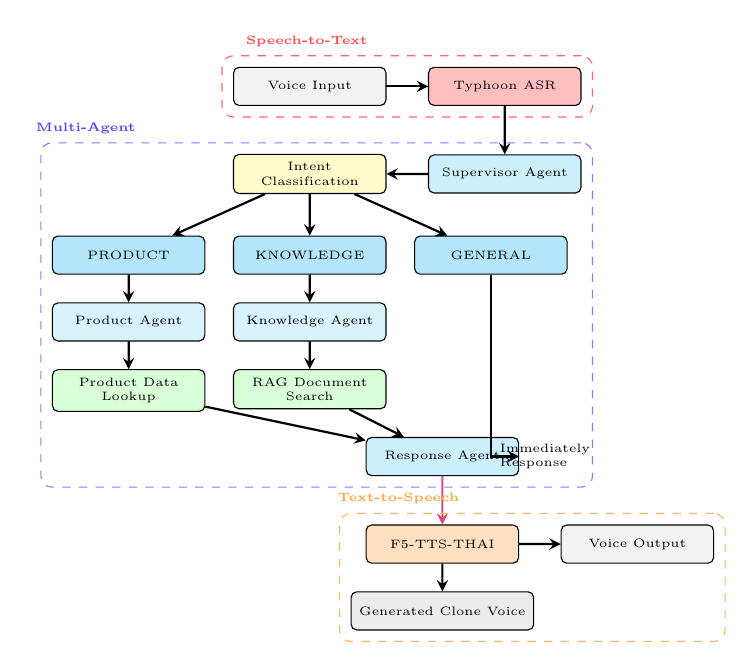
\begin{tikzpicture}[
        node distance=0.35cm and 0.45cm,
        scale=0.88,
        transform shape,
        box/.style={rectangle, draw, rounded corners=2pt, minimum width=2.2cm,
                    minimum height=0.55cm, align=center, font=\tiny},
        sectionbox/.style={rectangle, draw, dashed, rounded corners=4pt,
                           inner sep=4pt},
        arrow/.style={->, thick, >=stealth},
        darrow/.style={->, thick, >=stealth, draw=purple!70}
    ]

    %% SECTION 1: Speech-to-Text (ASR)
    \node[box, fill=gray!10] (voicein) {Voice Input};
    \node[box, fill=red!25, right=0.6cm of voicein] (asr) {Typhoon ASR};
    \draw[arrow] (voicein) -- (asr);
    \node[sectionbox, draw=red!60, fit=(voicein)(asr),
          label={[font=\tiny\bfseries, text=red!70]above left:Speech-to-Text}]
          (sec1) {};

    %% SECTION 2: Multi-Agent
    \node[box, fill=cyan!20, below=0.7cm of asr] (supervisor) {Supervisor Agent};
    \node[box, fill=yellow!20, left=0.6cm of supervisor] (intent)
          {Intent\\Classification};
    \draw[arrow] (asr) -- (supervisor);
    \draw[arrow] (supervisor) -- (intent);

    \node[box, fill=cyan!30, below left=0.6cm and 0.4cm of intent]
          (product) {PRODUCT};
    \node[box, fill=cyan!30, below=0.6cm of intent]
          (knowledge) {KNOWLEDGE};
    \node[box, fill=cyan!30, below right=0.6cm and 0.4cm of intent]
          (general) {GENERAL};
    \draw[arrow] (intent) -- (product);
    \draw[arrow] (intent) -- (knowledge);
    \draw[arrow] (intent) -- (general);

    \node[box, fill=cyan!15, below=0.4cm of product]   (pagent) {Product Agent};
    \node[box, fill=cyan!15, below=0.4cm of knowledge] (kagent) {Knowledge Agent};
    \draw[arrow] (product)   -- (pagent);
    \draw[arrow] (knowledge) -- (kagent);

    \node[box, fill=green!15, below=0.4cm of pagent]
          (pdatalookup) {Product Data\\Lookup};
    \node[box, fill=green!15, below=0.4cm of kagent]
          (ragsearch) {RAG Document\\Search};
    \draw[arrow] (pagent) -- (pdatalookup);
    \draw[arrow] (kagent) -- (ragsearch);

    \node[box, fill=cyan!20,
          below right=0.4cm and -0.3cm of ragsearch] (response) {Response Agent};
    \draw[arrow] (pdatalookup) -- (response);
    \draw[arrow] (ragsearch)   -- (response);
    \draw[arrow] (general) |- node[right, font=\tiny, align=left]
                                {Immediately\\Response} (response);

    \node[sectionbox, draw=blue!50,
          fit=(supervisor)(intent)(product)(knowledge)(general)
              (pagent)(kagent)(pdatalookup)(ragsearch)(response),
          label={[font=\tiny\bfseries, text=blue!70]above left:Multi-Agent}]
          (sec2) {};

    %% SECTION 3: Text-to-Speech (TTS)
    \node[box, fill=orange!25, below=0.7cm of response] (f5tts) {F5-TTS-THAI};
    \node[box, fill=gray!10, right=0.6cm of f5tts] (voiceout) {Voice Output};
    \draw[darrow] (response) -- (f5tts);
    \draw[arrow]  (f5tts)    -- (voiceout);

    \node[box, fill=gray!15, below=0.4cm of f5tts]
          (clonevoice) {Generated Clone Voice};
    \draw[arrow] (f5tts) -- (clonevoice);

    \node[sectionbox, draw=orange!60,
          fit=(f5tts)(voiceout)(clonevoice),
          label={[font=\tiny\bfseries, text=orange!70]above left:Text-to-Speech}]
          (sec3) {};

    \end{tikzpicture}
    \caption{System methodology overview. The pipeline consists of three stages:
    (1)~\textit{Speech-to-Text} transcribes voice input via Typhoon ASR;
    (2)~\textit{Multi-Agent} routing classifies intent and dispatches to
    Product, Knowledge, or General agents;
    (3)~\textit{Text-to-Speech} synthesises the final response via F5-TTS-THAI.}
    \label{fig:methodology}
\end{figure}

\begin{table}[h]
    \centering
    \caption{MANJU's four-tier architecture. Each tier runs in its own
             Docker container and can be scaled independently.}
    \label{tab:tiers}
    \small
    \begin{tabular}{@{}lll@{}}
        \toprule
        \textbf{Tier} & \textbf{Role} & \textbf{Key responsibilities} \\
        \midrule
        1 Frontend      & User interface     & React/TS workflow editor, voice capture, VAD \\
        2 API Gateway   & Security \& routing & Go server, Google OAuth, encrypted API keys \\
        3 AI Orchestrator & Reasoning        & LLM routing, RAG, Google Sheets integration \\
        4 TTS Service   & Voice synthesis    & Qwen3-TTS on GPU, three voice modes \\
        \bottomrule
    \end{tabular}
\end{table}

% -------------------------------------------------------------------
\subsection{ASR Module with Voice Activity Detection}
% -------------------------------------------------------------------

Speech recognition runs entirely in the browser via the Web Speech API
(\texttt{webkitSpeechRecognition}), so no audio is transmitted until the
utterance is complete.
A custom energy-based VAD continuously monitors microphone RMS energy and
triggers automatic query submission once silence exceeds
$\tau_\text{silence} = 1{,}100$\,ms (threshold $\theta_\text{VAD} = 0.01$),
providing a fully hands-free experience.

% -------------------------------------------------------------------
\subsection{How the Multi-Agent System Works}
% -------------------------------------------------------------------

The central idea behind MANJU is that a conversation workflow is treated
as a \textit{saved design}, not fixed software.
An operator arranges building blocks visually in the browser---much like
connecting puzzle pieces---to define how the system should handle different
questions.
This design is saved, and whenever a customer sends a query the system
automatically follows the operator's intended path to produce an answer.
No technical expertise is needed to change the behaviour: editing the
visual layout is all that is required.

\subsubsection{The Eight Building Blocks}

Workflows are assembled from eight component types grouped into four
categories, as listed in Table~\ref{tab:node_types}.
An operator combines these to create any conversation flow---for example,
``accept a spoken question, search the product catalogue, then speak the
answer aloud.''

\begin{table}[t]
    \centering
    \caption{The eight component types available in the MANJU workflow
             editor, grouped by what they do.}
    \label{tab:node_types}
    \small
    \begin{tabular}{@{}llp{3.8cm}@{}}
        \toprule
        \textbf{Category} & \textbf{Component} & \textbf{What it does} \\
        \midrule
        \multirow{2}{*}{Input}
          & Text input   & Accepts a typed message from the user \\
          & Voice input  & Accepts a spoken message via the browser \\
        \midrule
        \multirow{2}{*}{Processing}
          & AI model     & Asks an AI to understand the question and compose a reply \\
          & Branch       & Sends the conversation down different paths based on what was asked \\
        \midrule
        \multirow{2}{*}{Data}
          & Documents    & Searches uploaded files for relevant information \\
          & Google Sheets & Fetches live rows from a connected spreadsheet \\
        \midrule
        \multirow{2}{*}{Output}
          & Text output  & Returns the final answer as written text \\
          & Voice output & Reads the answer aloud in a chosen voice \\
        \bottomrule
    \end{tabular}
\end{table}

% -------------------------------------------------------------------
\subsection{How Documents Are Searched (RAG)}
% -------------------------------------------------------------------
\label{sec:rag}

To ground responses in operator-provided knowledge, MANJU employs
Retrieval-Augmented Generation (RAG)~\cite{lewis2020rag}.
Uploaded documents (PDF, DOCX, TXT) are split into overlapping
1{,}000-character chunks and embedded with
\texttt{text-embedding-3-small} (1{,}536-dimensional vectors) into a
persistent FAISS index.
At inference time, the user query is embedded and the top-3 nearest
chunks are retrieved and prepended to the LLM prompt as grounding
context, together with source filenames and similarity scores.

\subsection{Google Sheets Integration}

The \texttt{google-sheets} node fetches live spreadsheet data via \texttt{gspread} with OAuth2 authentication, converting it to a Markdown table (capped at 50 rows) and injecting it into the LLM prompt---enabling real-time access to inventory or pricing data without re-embedding.

\subsection{Text-to-Speech (TTS) Module}
\label{sec:tts}

Once the AI layer produces a text response, the TTS module converts it
into spoken audio and streams it back to the user.
MANJU supports two interchangeable providers selected inside the workflow
editor; Table~\ref{tab:tts_options} summarises their key differences.

% -------------------------------------------------------------------
\subsubsection{TTS Provider Comparison}
% -------------------------------------------------------------------

\begin{table}[h]
    \centering
    \caption{Comparison of the two TTS providers supported by MANJU.}
    \label{tab:tts_options}
    \small
    \begin{tabular}{@{}lll@{}}
        \toprule
        \textbf{Feature} & \textbf{OpenAI TTS} & \textbf{Qwen3-TTS} \\
        \midrule
        Deployment    & Cloud (external)   & On-premise (GPU) \\
        Data privacy  & Audio sent offsite & Stays in-house \\
        Setup         & API key only       & GPU required \\
        Thai voice cloning & No            & Yes \\
        Preset voices & 6 built-in         & 9 characters \\
        Best for      & Prototyping        & Production \\
        \bottomrule
    \end{tabular}
\end{table}

\noindent Qwen3-TTS additionally supports \textbf{VoiceDesign}: the
operator describes a desired voice in plain language (e.g.,
``young female, warm tone'') and the model generates it on the fly.
All three Qwen3-TTS variants are preloaded into GPU memory at startup
with Flash Attention~2~\cite{dao2022flashattention} and a brief warmup
pass, so switching between voice modes and serving the first request both
add no extra delay.

% -------------------------------------------------------------------
\subsubsection{How Audio Is Streamed Sentence by Sentence}
% -------------------------------------------------------------------

Synthesising an entire paragraph before playing anything would make the
system feel slow.
Instead, the response text is broken into short chunks --- at most
200 characters each --- and each chunk is synthesised and sent to the
browser independently.

\begin{itemize}[nosep]
    \item Thai text is split using PyThaiNLP's sentence
          tokeniser~\cite{pythainlp}.
    \item All other languages are split on standard sentence-ending
          punctuation.
    \item Very short fragments under 20 characters are merged with the
          next sentence to avoid sending near-empty audio clips.
\end{itemize}

\noindent The browser starts playing the first sentence while the server
is still generating the second and pre-fetching the third.
Completed audio clips are saved in the browser's local storage
(IndexedDB) so that repeating the same query plays back instantly
without re-synthesis.

% -------------------------------------------------------------------
\subsubsection{Measuring Speed: the Real-Time Factor}
% -------------------------------------------------------------------

Every response includes a speed metric called the Real-Time Factor (RTF),
defined as:

\begin{equation}
    \text{RTF} = \frac{t_\text{generation}}{t_\text{audio\_duration}}
    \label{eq:rtf}
\end{equation}

\noindent An RTF below 1.0 means the system generated the audio faster
than it takes to play it back --- in other words, faster than real time.
For example, an RTF of 0.42 means the server produced a 10-second audio
clip in only 4.2 seconds.
Each response also reports total generation time, pure model inference
time, audio duration, and the number of sentence chunks produced.
\subsection{Web Application}

\subsubsection{Visual Workflow Editor}
The workflow editor provides an infinite canvas with zoom/pan, drag-and-drop node placement from a template palette, cubic B\'{e}zier curve connection drawing, marquee multi-selection, and undo support.
Per-node-type configuration panels allow setting system prompts, model selection, RAG parameters, condition operators, TTS voice/provider, and output variable names.
The workflow is serialized as a JSON object containing \texttt{nodes[]} and \texttt{connections[]} arrays and persisted via the API gateway.

\begin{figure}[h]
    \centering
    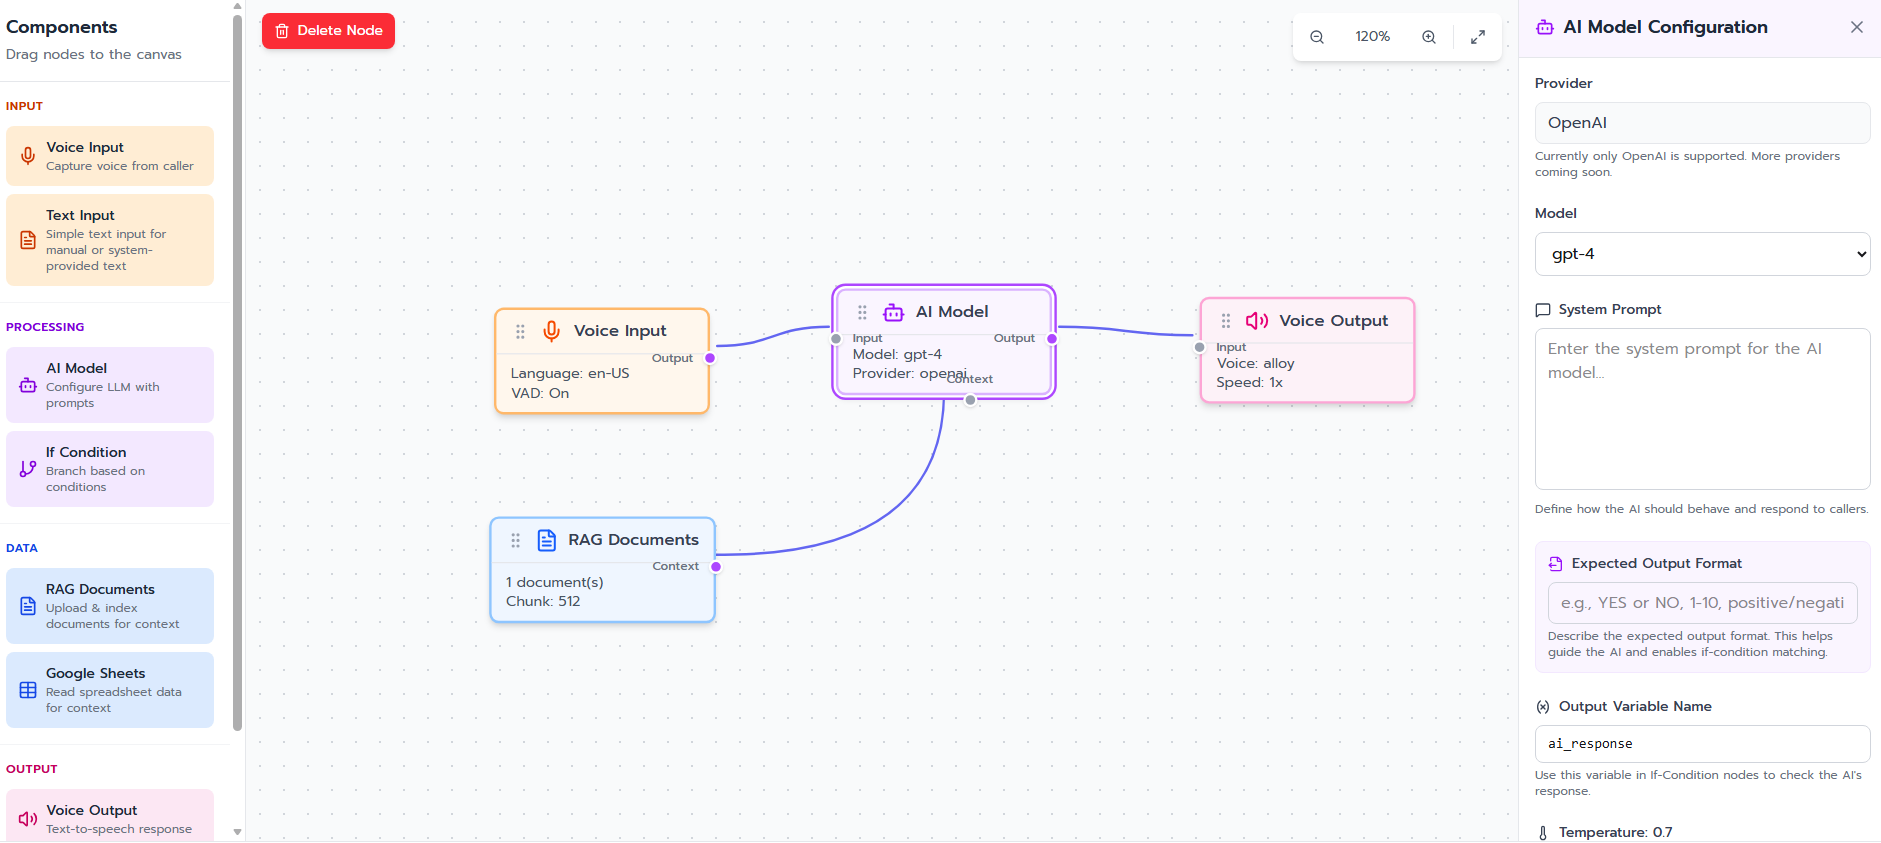
\includegraphics[width=\linewidth]{Node.png}
    \caption{Visual Workflow Editor showing the node canvas with drag-and-drop components,connections, and the AI Model configuration panel.}
    \label{fig:workflow_editor}
\end{figure}

\subsubsection{Demo Console and Voice Asset Management}
The demo console provides a chat interface for both text and voice I/O, displaying the ASR transcript in real time and playing synthesised audio with IndexedDB caching (keyed by a deterministic hash of text + voice settings) for instant replay.
Users may upload custom voice reference audio (WAV/MP3/M4A, max 50\,MB) for Qwen3-TTS cloning; files are stored in Azure Blob Storage or the local filesystem with metadata persisted in PostgreSQL.


% ===========================================================================
\section{Experiments}
\label{sec:experiments}
% ===========================================================================

\subsection{Experimental Setup}

We evaluate MANJU on a curated set of 50 Thai customer-service queries spanning three categories: FAQ (20 queries), product information (15 queries), and knowledge-base lookups (15 queries).
Each query has a reference answer prepared by domain experts.

\noindent\textbf{Hardware.}
The AI orchestrator runs on a CPU-only server (8-core, 32\,GB RAM).
Qwen3-TTS runs on an NVIDIA H100 80\,GB GPU with Flash Attention~2 enabled and all three model variants preloaded.

\noindent\textbf{Configuration.}
Default workflow: \texttt{voice-input} $\rightarrow$ \texttt{rag-documents} ($k{=}3$) $\rightarrow$ \texttt{ai-model} (GPT-4o-mini, $T{=}0.7$) $\rightarrow$ \texttt{voice-output} (Qwen3-TTS, CustomVoice).
RAG index contains 15 domain-specific PDF/DOCX documents (${\sim}$120 chunks after splitting).

\subsection{Metrics}

We report the following metrics:
\begin{enumerate}[label=(\roman*), nosep]
    \item \textbf{End-to-end latency} ($t_\text{e2e}$): time from query submission to first audio playback.
    \item \textbf{Component-level latency}: ASR ($t_\text{ASR}$), RAG retrieval ($t_\text{ret}$), LLM generation ($t_\text{LLM}$), and TTS first-sentence ($t_\text{TTS}$).
    \item \textbf{Time-to-first-token} (TTFT): latency from prompt submission to first LLM output token.
    \item \textbf{TTS Real-Time Factor} (RTF): as defined in Eq.~\eqref{eq:rtf}.
    \item \textbf{TTS intelligibility} (WER): word error rate from re-transcribing synthesised audio with Whisper.
    \item \textbf{TTS naturalness} (MOS): mean opinion score (1--5) from three native Thai-speaking annotators on 10 sampled responses.
    \item \textbf{Intent routing accuracy}: percentage of queries routed to the correct agent node.
    \item \textbf{Answer groundedness}: percentage of responses whose key claims are supported by retrieved RAG passages, judged by two human annotators.
\end{enumerate}

\subsection{Baselines}

We compare three RAG configurations and three LLM backends.

\noindent\textbf{RAG Configurations:}
\begin{enumerate}[label=(\alph*), nosep]
    \item \textbf{Full pipeline:} Multi-agent workflow with RAG + Qwen3-TTS (proposed system).
    \item \textbf{Single-agent:} Direct LLM inference without workflow routing or RAG.
    \item \textbf{No-RAG:} Multi-agent workflow with RAG nodes removed (LLM-only generation).
\end{enumerate}

\noindent\textbf{LLM Backends} (full pipeline, same RAG and TTS):
\begin{enumerate}[label=(\roman*), nosep]
    \item \textbf{GPT-4o-mini} (cloud, default): strong instruction following at low cost.
    \item \textbf{Qwen2.5-7B-Instruct} (on-premise): open-weight, data stays on infrastructure.
    \item \textbf{GPT-4o} (cloud, upper bound): highest-capability reference.
\end{enumerate}

\subsection{Results}

\subsubsection{Latency Analysis}

Table~\ref{tab:latency} presents the mean latency breakdown across the evaluation set.

\begin{table}[t]
    \centering
    \caption{Mean latency breakdown (seconds) across 50 evaluation queries. $t_\text{ret}$ and $t_\text{LLM}$ are sub-components of orchestration; $t_\text{TTS}$ is measured to first sentence playback.}
    \label{tab:latency}
    \small
    \resizebox{\columnwidth}{!}{%
    \begin{tabular}{@{}lcccccc@{}}
        \toprule
        \textbf{Config.} & $t_\text{ASR}$ & $t_\text{ret}$ & $t_\text{LLM}$ & TTFT & $t_\text{TTS}$ & $t_\text{e2e}$ \\
        \midrule
        Full pipeline & 0.8 & 0.3 & 1.8 & 0.4 & 1.8 & 4.7 \\
        Single-agent  & 0.8 & ---  & 1.4 & 0.4 & 1.8 & 4.0 \\
        No-RAG        & 0.8 & ---  & 1.2 & 0.4 & 1.8 & 3.8 \\
        \bottomrule
    \end{tabular}%
    }
\end{table}

\noindent The full pipeline achieves a mean $t_\text{e2e}$ of 4.7\,s, within the 5-second design target.
RAG retrieval adds only $t_\text{ret}{=}0.3$\,s; the dominant cost is LLM generation ($t_\text{LLM}{=}1.8$\,s), with TTFT of 0.4\,s confirming fast streaming onset.
Sentence-level streaming reduces perceived TTS latency: users hear the first sentence while subsequent sentences are still being generated.

\subsubsection{TTS Quality and Speed}

Table~\ref{tab:tts_quality} reports Qwen3-TTS-12Hz-1.7B quality and speed on the H100 GPU with Flash Attention~2.
The system achieves faster-than-real-time synthesis (RTF\,=\,0.42) with high intelligibility (WER\,=\,3.1\%) and natural-sounding Thai output (MOS\,=\,4.1\,/\,5.0).
Voice cloning preserves speaker identity well (speaker similarity\,=\,0.87), and the multi-model cache eliminates switching overhead between voice modes.

\begin{table}[h]
    \centering
    \caption{TTS quality and speed evaluation (Qwen3-TTS-12Hz-1.7B, H100 GPU, CustomVoice mode, 50 responses).}
    \label{tab:tts_quality}
    \small
    \begin{tabular}{@{}llc@{}}
        \toprule
        \textbf{Metric} & \textbf{Description} & \textbf{Value} \\
        \midrule
        RTF                    & Generation / audio duration            & 0.42 \\
        First-sentence latency & Time to first audio chunk              & 1.8\,s \\
        WER (round-trip)       & Whisper re-transcription error rate    & 3.1\% \\
        MOS-Naturalness        & 3 native Thai speakers, scale 1--5     & 4.1\,/\,5.0 \\
        Speaker Similarity     & ECAPA-TDNN cosine sim.\ (cloning mode) & 0.87 \\
        \bottomrule
    \end{tabular}
\end{table}

\subsubsection{LLM Backend Comparison}

Table~\ref{tab:llm_compare} compares the three LLM backends on the full pipeline.
GPT-4o-mini offers the best cost--accuracy trade-off and is the default choice.
Qwen2.5-7B-Instruct provides a viable on-premise alternative at zero API cost, with a modest drop in routing accuracy (88\%) and groundedness (82\%).
GPT-4o serves as the capability ceiling, improving routing to 96\% at a $10\times$ cost increase.

\begin{table}[h]
    \centering
    \caption{LLM backend comparison on the full pipeline (50 queries). Cost is estimated USD per query at standard API pricing.}
    \label{tab:llm_compare}
    \small
    \resizebox{\columnwidth}{!}{%
    \begin{tabular}{@{}lcccc@{}}
        \toprule
        \textbf{LLM} & \textbf{Routing Acc.} & \textbf{Grounded} & \textbf{TTFT (s)} & \textbf{Cost/Query} \\
        \midrule
        GPT-4o-mini (default) & 94.0\% & 88.0\% & 0.4 & \$0.0003 \\
        Qwen2.5-7B-Instruct   & 88.0\% & 82.0\% & 0.9 & \$0.00 \\
        GPT-4o (upper bound)  & 96.0\% & 91.0\% & 0.6 & \$0.0032 \\
        \bottomrule
    \end{tabular}%
    }
\end{table}

\subsubsection{Routing and Groundedness}

\begin{table}[t]
    \centering
    \caption{Intent routing accuracy and answer groundedness (\%) across evaluation categories.}
    \label{tab:accuracy}
    \small
    \resizebox{\columnwidth}{!}{%
    \begin{tabular}{@{}lccc@{}}
        \toprule
        \textbf{Category} & \textbf{Routing Acc.} & \textbf{Grounded (Full)} & \textbf{Grounded (No-RAG)} \\
        \midrule
        FAQ       & 95.0 & 90.0 & 60.0 \\
        Product   & 93.3 & 86.7 & 46.7 \\
        Knowledge & 93.3 & 86.7 & 40.0 \\
        \midrule
        \textbf{Overall} & \textbf{94.0} & \textbf{88.0} & \textbf{50.0} \\
        \bottomrule
    \end{tabular}%
    }
\end{table}

\noindent Table~\ref{tab:accuracy} shows that the conditional routing mechanism achieves 94\% accuracy in directing queries to the appropriate processing path.
RAG grounding improves answer groundedness from 50\% (No-RAG) to 88\% (Full pipeline), demonstrating the critical impact of retrieval on factual accuracy.

\subsubsection{Failure Analysis}
Common failure modes include: (i)~ASR misrecognition of domain-specific Thai terminology (3 of 50 queries), (ii)~ambiguous queries that trigger incorrect conditional routing (3 of 50), and (iii)~missing knowledge where the RAG index does not contain relevant documents (2 of 50).

\subsection{Discussion}

The workflow-as-data architecture enables rapid domain adaptation: adding a new FAQ category requires only uploading documents and optionally adding a conditional branch in the visual editor, without code changes or redeployment.
The dual-TTS architecture provides flexibility: OpenAI TTS for quick prototyping and Qwen3-TTS for production deployments requiring voice cloning and GPU-accelerated Thai synthesis.

The sentence-level streaming strategy is critical for user experience: even though total TTS generation for a full response may take 3--4 seconds, the user hears the first sentence within 1.8 seconds, creating a perception of responsiveness.
The IndexedDB caching layer further eliminates TTS latency on repeated queries.

% ===========================================================================
\section{Conclusion}
\label{sec:conclusion}
% ===========================================================================

This paper presented MANJU, an end-to-end Thai voice-based customer-service platform combining browser-based ASR with VAD, LangGraph multi-agent orchestration with RAG grounding, and GPU-accelerated Qwen3-TTS with voice cloning.
The workflow-as-data architecture allows non-technical users to visually compose agent topologies without code changes.
Experimental evaluation demonstrates sub-5-second end-to-end latency, 94\% intent routing accuracy, and 88\% answer groundedness with RAG enabled, significantly outperforming configurations without retrieval.

\noindent\textbf{Future Work.}
Key directions include: (i)~replacing browser-based ASR with server-side Typhoon ASR Real-Time~\cite{sirichotedumrong2026typhoonasr} for lower CER on Thai domain terms and on-premises privacy, (ii)~supporting multi-turn stateful conversations with workflow-level memory, and (iii)~parallelising orchestration node execution to reduce latency on complex graphs.

% ===========================================================================
% References
% ===========================================================================
\bibliographystyle{IEEEtran}
\bibliography{references}

\end{document}